\documentclass[5p]{elsarticle}        % 5p gir 2 kolonner pr side. 1p gir 1 kolonne pr side.
\journal{fagl\ae rer}
\usepackage[T1]{fontenc} 				% Vise norske tegn.
\usepackage[norsk]{babel}				% Tilpasning til norsk.
\usepackage[utf8]{inputenc}             % selv puttet inn for � kunne skrive norske tegn
\usepackage{graphicx}       				% For � inkludere figurer.
\usepackage{amsmath,amssymb} 				% Ekstra matematikkfunksjoner.
\usepackage{siunitx}					% M� inkluderes for blant annet � f� tilgang til kommandoen \SI (korrekte m�ltall med enheter)
	\sisetup{exponent-product = \cdot}      	% Prikk som multiplikasjonstegn (i steden for kryss).
 	\sisetup{output-decimal-marker  =  {,}} 	% Komma som desimalskilletegn (i steden for punktum).
 	\sisetup{separate-uncertainty = true}   	% Pluss-minus-form p� usikkerhet (i steden for parentes). 
\usepackage{booktabs}                     		% For � f� tilgang til finere linjer (til bruk i tabeller og slikt).
\usepackage[font=small,labelfont=bf]{caption}		% For justering av figurtekst og tabelltekst.
\usepackage{comment}                            % for � kunne kommentere i bolker (med \begin{comment} og \end{comment})
\usepackage[export]{adjustbox}            % for � kunne plassere figurer bedre, h�yre venstre justering
\usepackage[below]{placeins}                      %tillatter bruk av \FloatBarrier ([above], [below])
\usepackage{pdfpages}

%\usepackage[section]{below}        %begrenser figuerer til sin section, kan bruker i stedet for \usepackage{placeins} 

% Denne setter navnet p� abstract til Sammendrag
\renewenvironment{abstract}{\global\setbox\absbox=\vbox\bgroup
\hsize=\textwidth\def\baselinestretch{1}%
\noindent\unskip\textbf{Sammendrag}
\par\medskip\noindent\unskip\ignorespaces}
{\egroup}


% Disse kommandoene kan gj�re det enklere for LaTeX � plassere figurer og tabeller der du �nsker.
\setcounter{totalnumber}{5}
\renewcommand{\textfraction}{0.05}
\renewcommand{\topfraction}{0.95}
\renewcommand{\bottomfraction}{0.95}
\renewcommand{\floatpagefraction}{0.35}

%%%%%%%%%%%%%%%%%%%%%%%%%%%%%%%%%%%%%%%%%%%%%%%%%%%%%%%%%%%%%%%%%%%%%%%%%
\begin{document}
\begin{frontmatter}
\title{}
\author[fysikk]{H\aa kon Task{\'{e}}n}
\author[fysikk]{Paul Thrane}
%\address[fysikk]{Institutt for fysikk, Norges Teknisk-Naturvitenskapelige Universitet, N-7491 Trondheim, Norway.}
\begin{abstract}


\end{abstract}
\end{frontmatter}
%%%%%%%%%%%%%%%%%%%%%%%%%%%%%%%%%%%%%%%%%%%%%%%%%%%%%%%%%%%%%%%%%%%%%%%%%
%\section{Innledning}



%%%%%%%%%%%%%%%%%%%%%%%%%%%%%%%%%%%%%%%%%%%%%%%%%%%%%%%%%%%%%%%%%%%%%%%%%
\section{Teori og metode}
Bevegelsen til en partikkel i posisjon $\vec{r}_i$ med masse $m_i$, utsatt for en kraft $\vec{F}_i$, vil v\ae re bestemt av Newtons bevegelsesligning
\begin{equation}
m_i\frac{\mathrm{d}^2\vec{r}_i}{\mathrm{d}t^2}=\vec{F}_i.
\label{N2}
\end{equation}
Ligning \eqref{N2} kan skrives om til to koblede differensialligninger \cite{prosjektbeskrivelse}
\begin{equation}
\frac{\mathrm{d}\vec{v}_i}{\mathrm{d}t} = \vec{f}_i,
\label{n1}
\end{equation}
\begin{equation}
\frac{\mathrm{d}\vec{r}_i}{\mathrm{d}t}  = \vec{v}_i,
\label{n2}
\end{equation}
hvor $\vec{f}_i$ er kraft per masse p\aa \ partikkelen og $\vec{v}_i$ er hastigheten til partikkelen. Dersom initialbetingelser for $\vec{r}_i$ of $\vec{v}_i$ er kjent kan videre tidsforl\o p bestemmes ved numerisk l\o sning av \eqref{n1} og \eqref{n2} hvis $\vec{f}_i$ kan beregnes p\aa \ grunnlag av posisjon og hastighet til partikkelen. En metode som kan benyttes til dette er Verlet integrasjon, hvor $\vec{r}_i(t + \Delta t)$ og  $\vec{v}_i(t + \Delta t)$ beregnes etter kjennskap til $\vec{r}_i(t)$ ved f\o lgende ligninger\cite{prosjektbeskrivelse}
\begin{equation}
\vec{v}_i(t + \frac{\Delta t}{2}) = \vec{v}_i(t) + \vec{f}_i(t)\frac{\Delta t}{2},
\end{equation}
\begin{equation}
\vec{r}_i(t + \Delta t) = \vec{r}_i(t) + \vec{v}_i(t + \frac{\Delta t}{2})\Delta t,
\end{equation}
\begin{equation}
\vec{v}_i(t + \Delta t) = \vec{v}_i(t + \frac{\Delta t}{2}) + \vec{f}_i(t + \Delta t)\frac{\Delta t}{2}.
\end{equation}

Dersom potensialet til partikkelen, $V_i$, er kjent, kan kraften p\aa \ partikkelen beregnes ut fra sammenhengen $\vec{F}_i=-\nabla V_i$. I dette numeriske fors\o ket ble Verlet integrasjon benyttet for \aa \ beregne bevegelsene til \'{e}n og to massive partikler i bane rundt et sentralt legeme med masse $M$ og med gravitasjon som eneste vekselvirkende kraft. Det ble antatt at partiklenes masse, $m_1$ og $m_2$, var mye mindre enn $M$ slik at den sentrale massen st\aa r fast i origo. For \'{e}n enkelt partikkel blir potensialet
\begin{equation}
V_1 = \frac{GMm_1}{r_1},
\end{equation}
med $G$ en konstant som bestemmer styrken p\aa \ gravitasjonskraften. For to partikler blir potensialet p\aa \ partikkel $i$ ogs\aa \ p\aa virket av posisjonen til partikkel $j$
\begin{equation}
V_i = \frac{GMm_i}{r_i} + \frac{Gm_im_j}{r_i-r_j}.
\end{equation}

For \aa \ unders\o ke n\o yaktignheten av den numeriske metoden ble bevaring av energi og dreieimpuls unders\o kt. I tillegg ble de beregnede orbitalene til en enkelt partikkel sammenlignet med det eksakte uttrykket \cite{goldstein}
\begin{equation}
r = \frac{a(1-e^2)}{1+e\cos{(\theta - \theta')}},
\end{equation}
hvor $(r,\theta)$ er posisjonen til partikkelen i polarkoordinater. Konstantene $a = -GM/2E$, og $e=(1+2El^2/m_1G^2M^2)^{0.5}$, der $E$ er energien til partikkelen og $l$ er dreieimpulsen om origo. Konstanten $\theta'$ spesifiseres av initialbetingelsene og kan settes lik null om en kun er interessert i hele orbitalen. Videre ble ogs\aa \ virialteoremet for \aa \ unders\o ke n\o yaktigheten av metoden da den gir en sammenheng mellom gjennomsnittlig kinetisk energi $\bar{T}$ og gjennomsnittlig potensiell energi $\bar{V}$ for en partikkel i et sentralt gravitasjonsfelt gitt ved\cite{goldstein}
\begin{equation}
\frac{\bar{T}}{\bar{V}}=-\frac{1}{2}.
\label{virial}
\end{equation}
Koden som er blitt benyttet for \aa \ l\o se ligning \eqref{n1} og \eqref{n2} er i appendix.
%%%%%%%%%%%%%%%%%%%%%%%%%%%%%%%%%%%%%%%%%%%%%%%%%%%%%%%%%%%%%%%%%%%%%%%%%
\section{Resultat}
For kun en partikkel gir metoden en godt definert ellipseformet orbital. Figur \ref{1pos} viser resultatet av en simulasjon sammen med tilh\o rende eksakte l\o sning. Ved \aa \ teste for ulike inertialbetingelser ble det funnet at et tidsteg p\aa \ under en promille av beregnet oml\o pstid som regel resulterte i en endring av total energi i st\o rrelsesorden $0.01\%$, mens et tidssteg p\aa \ omtrent $1\%$ av beregnet oml\o pstid resulterte i en endring av energi i st\o rrelsesorden $1\%$. Figur \ref{1energi} viser tilh\o rende total energi som funksjon av tid for systemet vist i figut \ref{1pos}.

eksakt losning,

$\bar{T}$ og \bar{V}

For to vekselvirkende partikler i et sentralt gravitasjonsfelt ble n\o yaktigheten d\aa ligere. Dersom initialbetingelsene f\o rte partiklene i n\ae rheten av hverandre ble det ofte store avvik i total energi og ustabile orbitaler. Dersom initialbetingelsene ble bestemt slik at partiklene ikke kom for n\ae rme hverandre ble imidlertid banene ganske stabile, men med en regelmessig forskyvning av orbitalen il\o pet av simuleringen, figur \ref{2pos} viser et slikt tilfelle. Figur \ref{2energi} viser total energi som funksjon av tid for samme simulering, som p\aa \ det meste avviker $0.20\%$ fra startenergi. Endring av total dreieimpuls for samme simulering var for liten til \aa \ kunne leses av, noe som ogs\aa \ gjaldt andre simuleringer uten store avvik av total energi.
\begin{figure}[h] 
	\begin{center}
		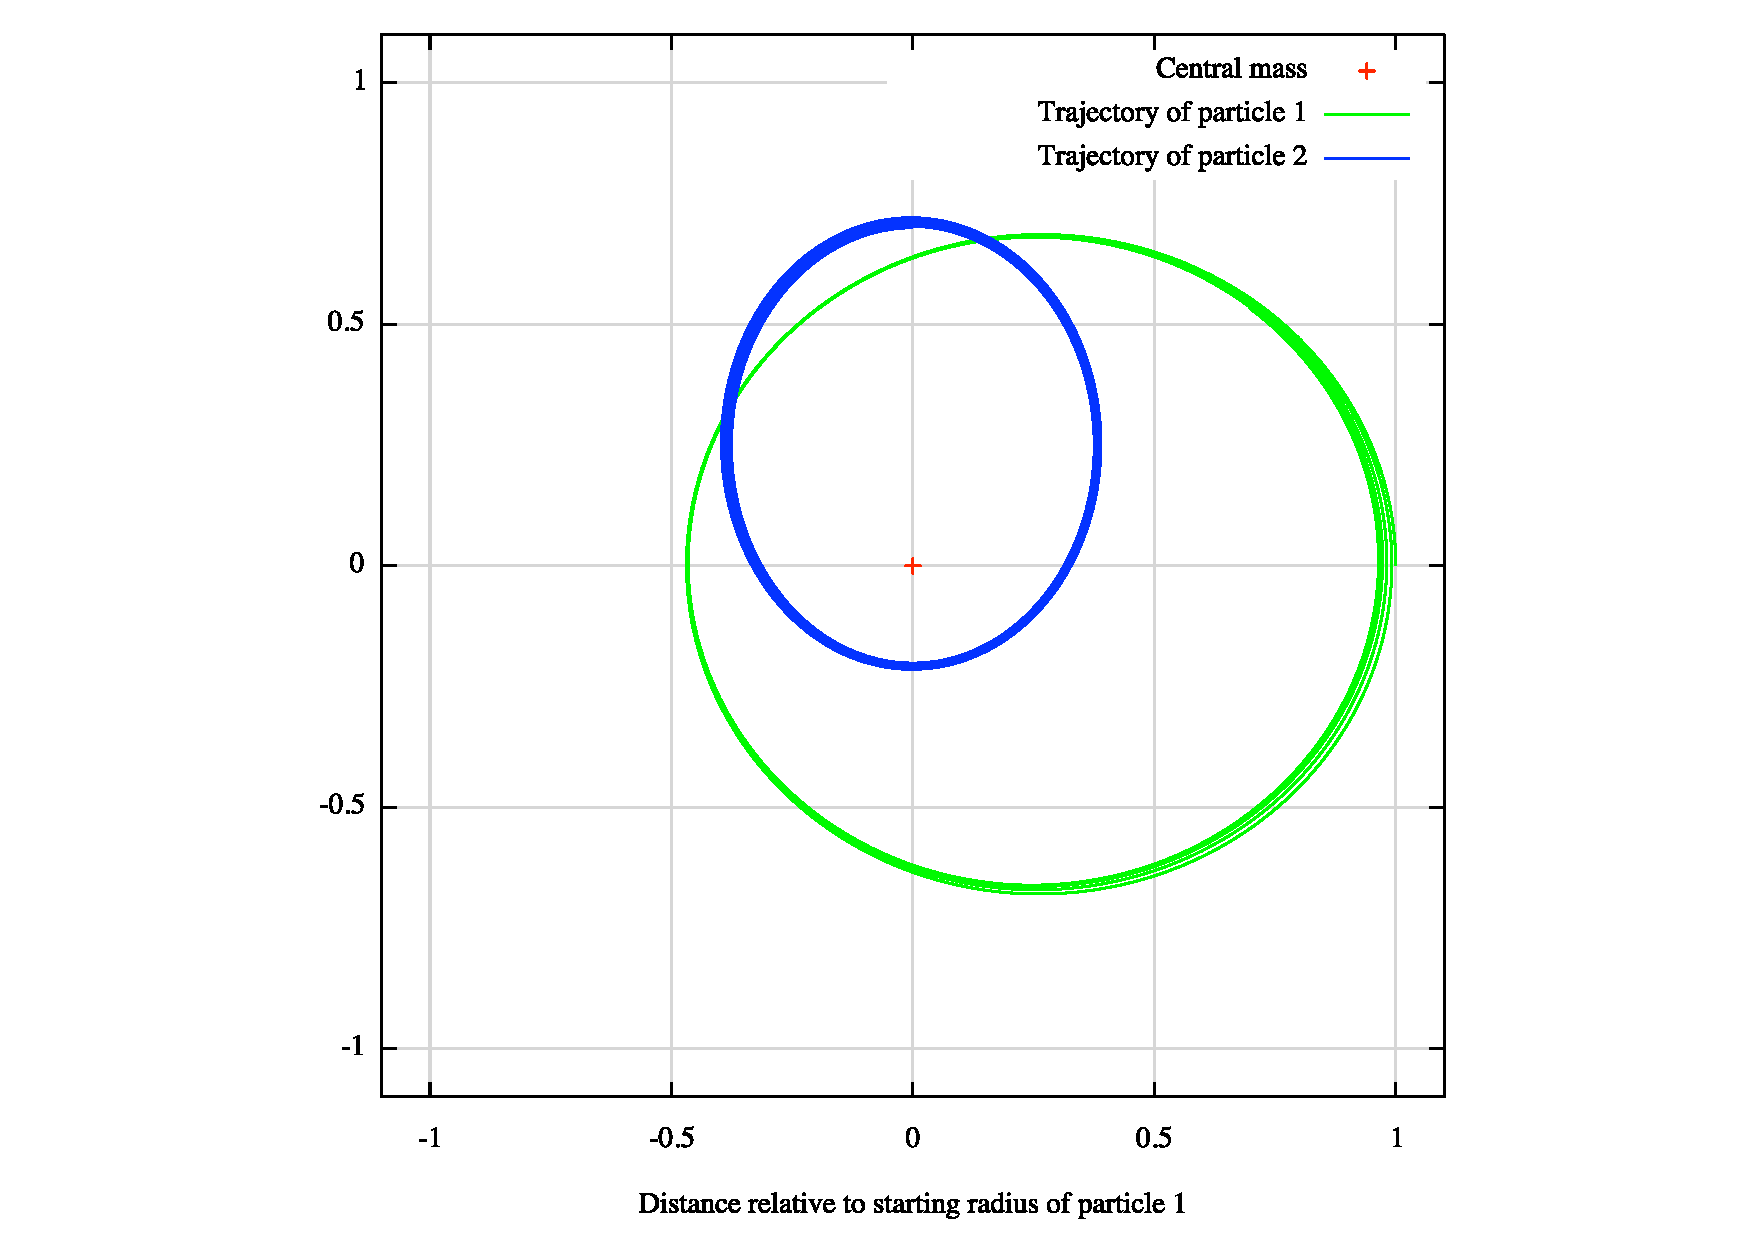
\includegraphics[width=.55\textwidth,center]{two_particles_position.pdf} 
	\end{center}
		\caption{Bevegelse for to vekselvirkende partikler i et sentralt gravitasjonsfelt. Partikkel 1 g\aa r mot klokken med oml\o pstid 3,8, partikkel 2 g\aa r mot klokken med oml\o pstid 1,8.} 
		\label{2pos} % Som med ligningen, er dette navnet vi refererer til.
\end{figure}
\begin{figure}[h] 
	\begin{center}
		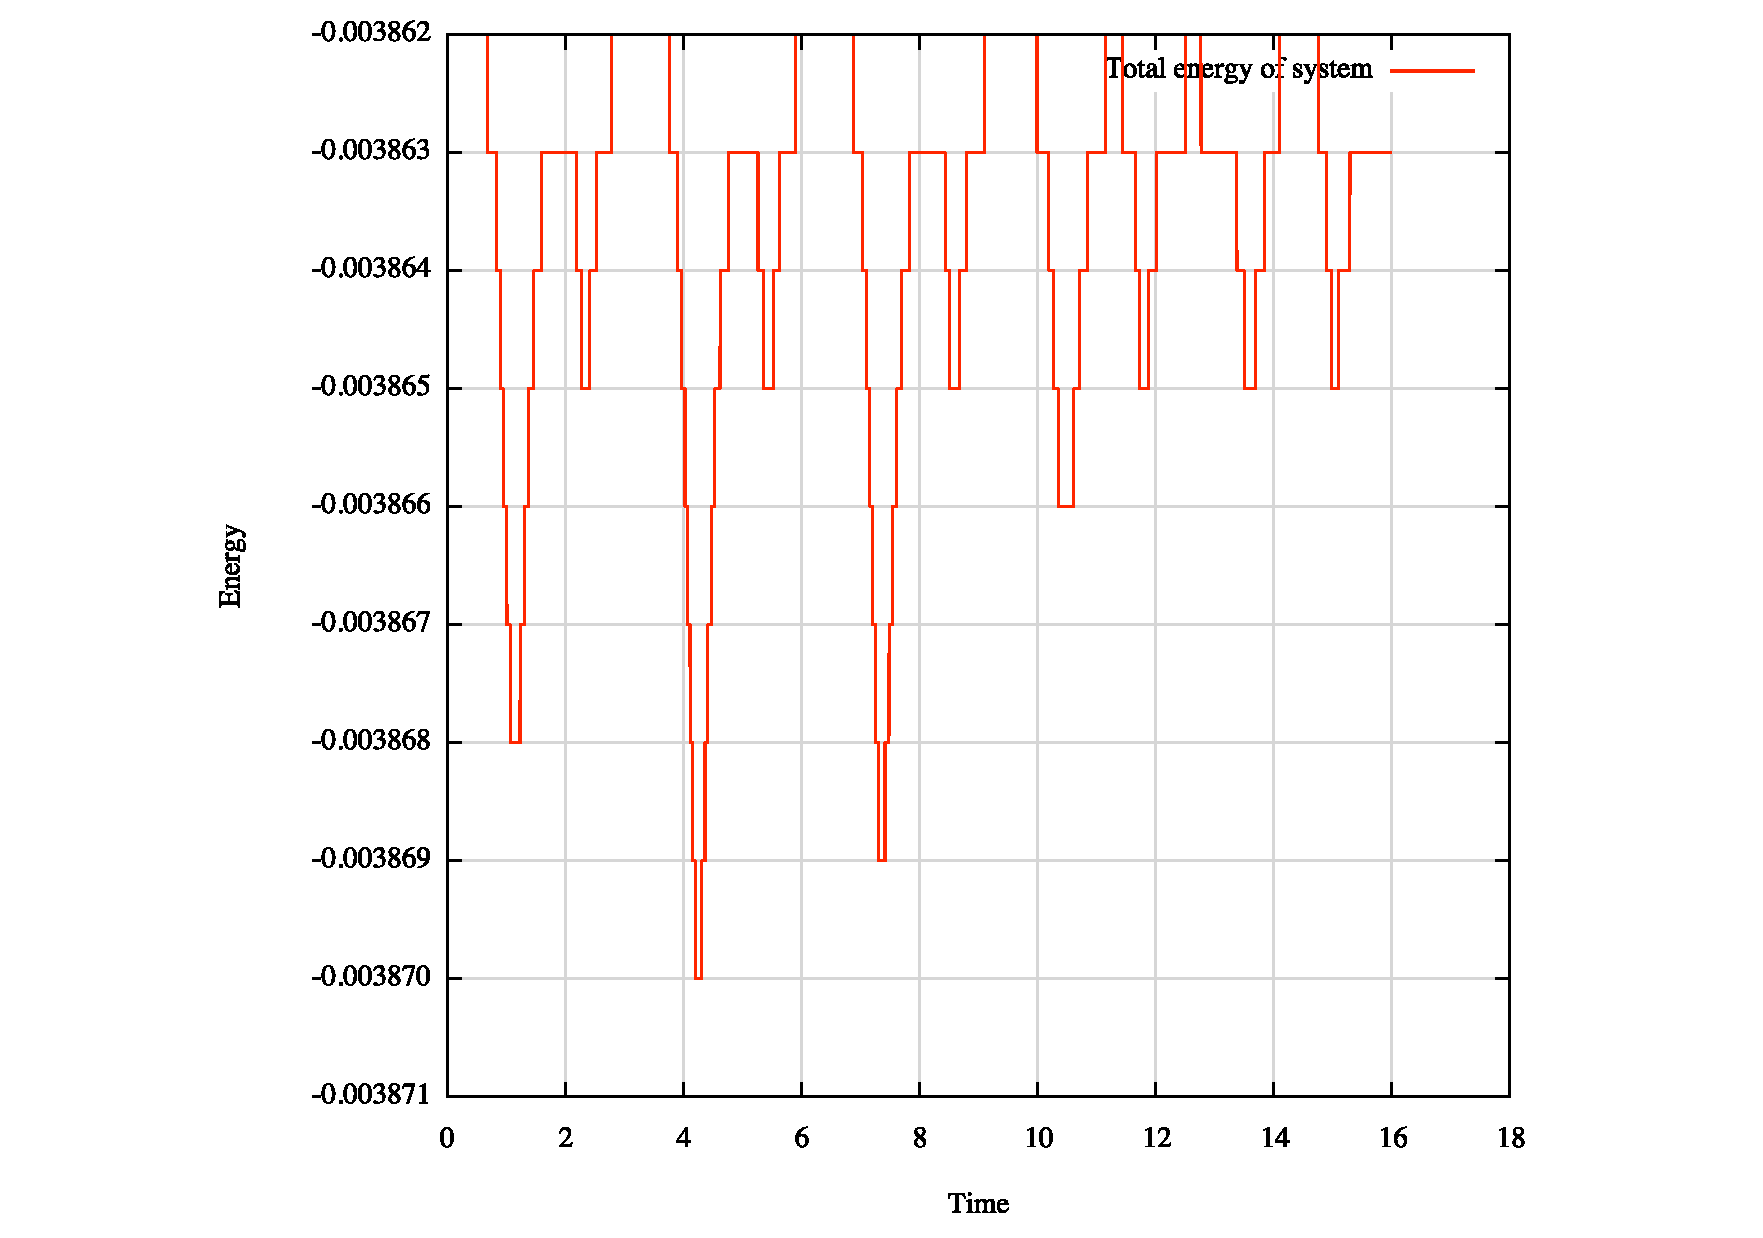
\includegraphics[width=.55\textwidth,center]{two_particles_energy.pdf} 
	\end{center}
		\caption{Total energi for system av to vekselvirkende partikler i et sentralt gravitasjonsfelt. Viser tidsforl\o p for system vist i figur \ref{2pos}} 
		\label{2energi} % Som med ligningen, er dette navnet vi refererer til.
\end{figure}

%%%%%%%%%%%%%%%%%%%%%%%%%%%%%%%%%%%%%%%%%%%%%%%%%%%%%%%%%%%%%%%%%%%%%%%%%
\section{Diskusjon}
Feil st\o rst n\ae rme origo

For to partikler blir metoden un\o yaktig hvis partiklene kommer i n\ae rheten av hverande. Dersom de holder en viss avstand f\aa r partiklene stabile orbitaler som er er svakt forskj\o vet, men selv i dette tilfellet blir total energi endret i intervallene der de er n\ae rmest. Dette kan sees i figur \ref{2energi}, der avvikene i total energi skjer i de omr\a dene der banen til partikkel 1 overlapper med banen til partikkel 2, se figur \ref{2pos}.
%%%%%%%%%%%%%%%%%%%%%%%%%%%%%%%%%%%%%%%%%%%%%%%%%%%%%%%%%%%%%%%%%%%%%%%%%
\section{Konklusjon}

%%%%%%%%%%%%%%%%%%%%%%%%%%%%%%%%%%%%%%%%%%%%%%%%%%%%%%%%%%%%%%%%%%%%%%%%%
\section*{Referanser}

\begin{thebibliography}{99}

\bibitem{prosjektbeskrivelse}
Prosjektbeskrivelse, Classical Mechanics TFY4345 - Computational Physics Project. NTNU, H\o sten 2015.

\bibitem{goldstein}
Goldstein, Safko, Poole. Classical Mechanics. Pearson Education Limited, Pearson new international edition, 3. utgave, 2014.

\end{thebibliography}

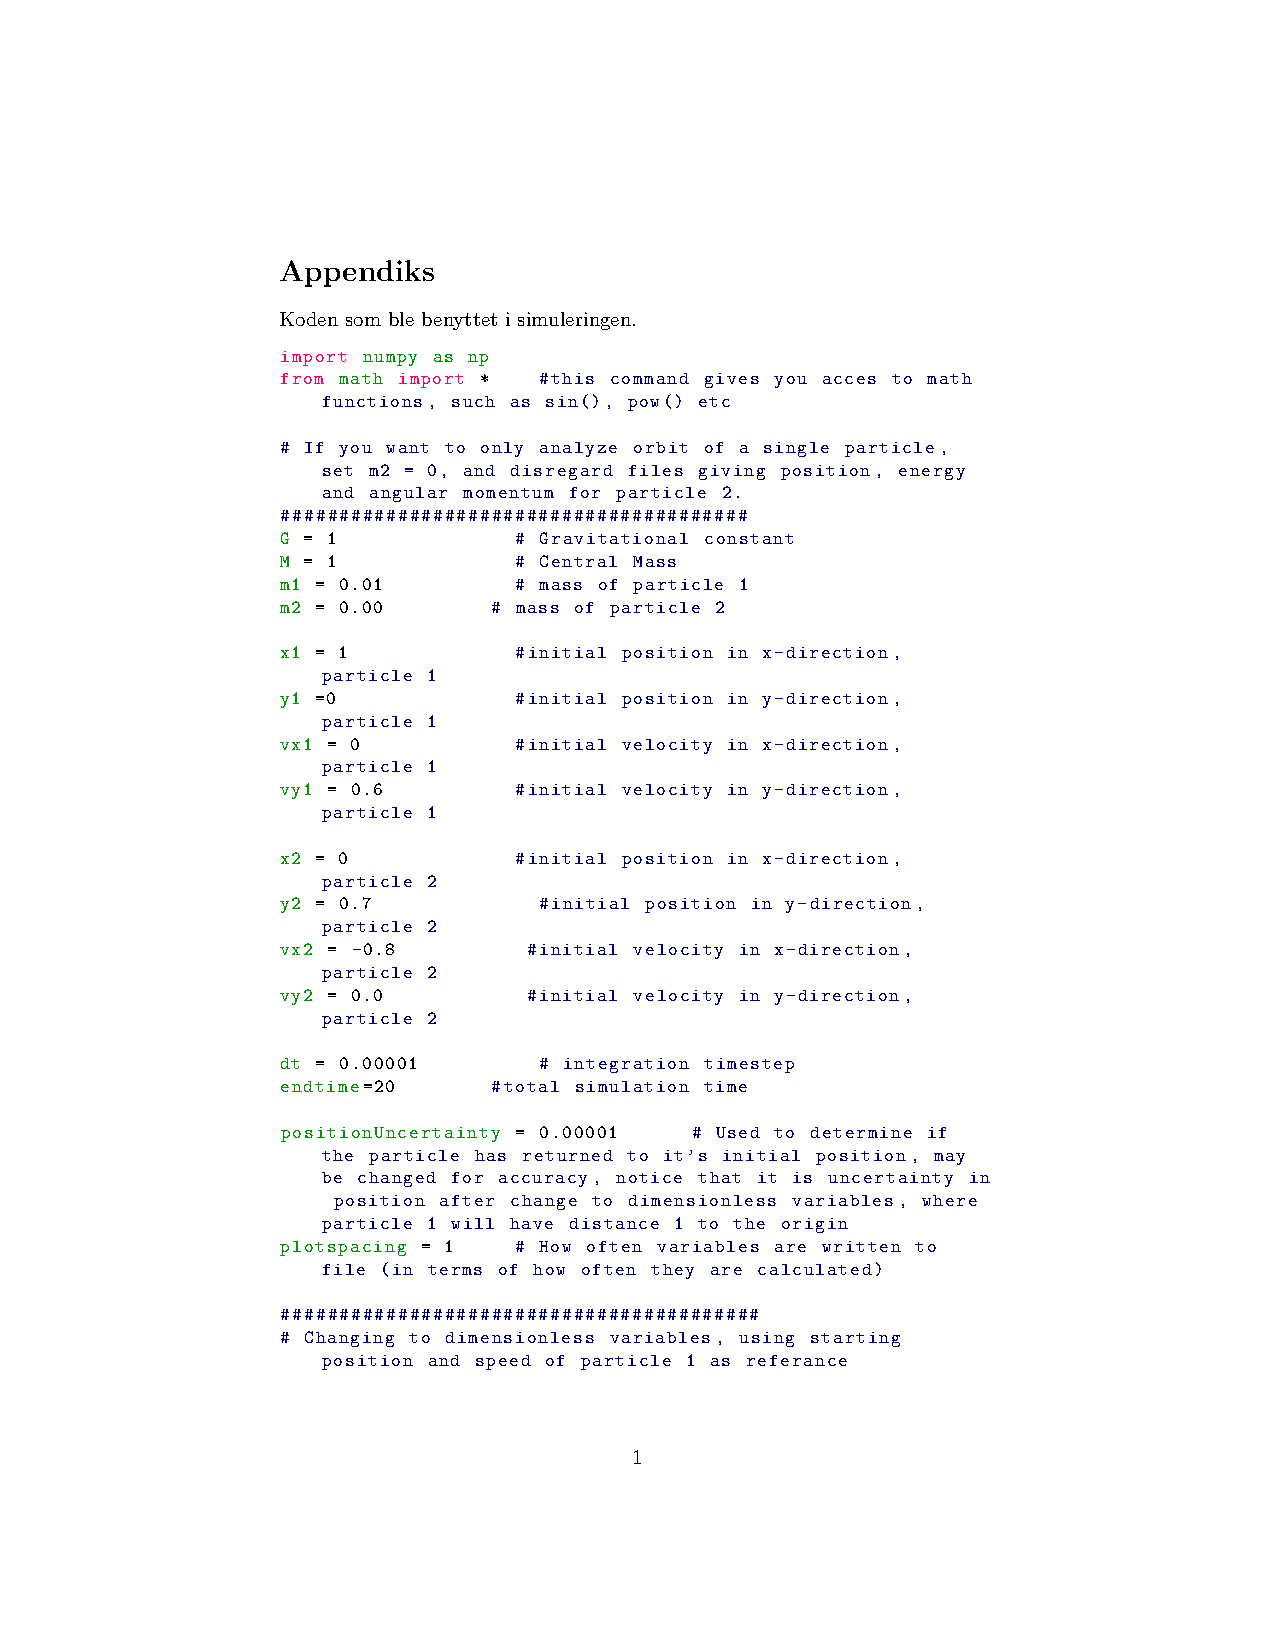
\includepdf[pages={1-},scale=1.2]{Appendix.pdf}


\end{document}